%%%%%%%%%%%%%%%%%%%%%%%%%%%%%%%%%%%%%%%%%%%%%%%%%%%%%%%
% Copied from previous \section{Neural Network Training}
In the VBF-enriched \TwoJet category, a DNN-based binary classifier is used as a final discriminant.
This section describes how this DNN, referred to as \emph{VBF DNN} in the following, is developed using supervised learning with simulated $pp$ collision events.
The relevant ML concepts are introduced in \cref{chap:ml}.
The DNN is developed using industry-standard open-source ML libraries, integrated in a self-developed software framework that has been continuously developed during the course of the author's PhD to manage the full ML cycle efficiently. The entire software suite used is summarized in \cref{app:software-suite}.

\subsection{Methodology and historical developments}
Implementing a neural network model into a physics analysis is a multi-stage procedure. 

\paragraph{Stage 1}
The first step is to prepare the training data.
The simulated samples that are listed in \cref{subsec:simulated-event-samples} are therefore transformed in a way, so they can be easily used with state-of-the-art ML software. Details on the training data are given in \cref{subsec:training-data}

\paragraph{Stage 2}
The second stage is the main part of the DNN development and involves the training, validation, and optimization of the DNN. The details of this iterative workflow are presented in \cref{subsec:hyper-parameters}.

\paragraph{Stage 3}
The third step is to deploy the neural network in the \HWW\ analysis and produce final measurement results. This ultimately demonstrates the final performance of the trained DNN model, and reveals the weak-spots of the analysis and the developed model. The latter information can be used to adapt the training procedure in stage two and further improve the DNN model. 
How this was done for the VBF DNN is described in \cref{subsec:sample-fraction-optimization}.

\paragraph{Final model selection}
The final DNN model is selected when no further improvements can be made by repeating step two and three. It should be noted that the tasks involved in step three are very time-consuming and computing-expensive, which limits the number of cycles that can realistically be carried out.
It should also be noted that the training procedure has been modified several times during the course of the author's PhD, due to both improvements in the self-developed software and historical developments of the \HWW\ analysis (for example changes in MC simulated samples). If not mentioned otherwise, the results and procedures presented correspond to the final VBF DNN. 
% that improvements of the self-developed software, together with historical developments of the entire \HWW\ analysis, lead to several modifications of the training setup over time. 

% During the course of the author's doctoral studies, some approaches have evolved, which means that certain parts of the training procedure have been optimized based on earlier versions of the training setup than the version used for the final DNN. 
% The following outlines roughly the different stages of the training, to motivate the procedures and decisions that were taken that resulted in the development of the final DNN used in this analysis. 
% The hyperparameters and procedure used for the final DNN are summarized in \cref{tab:hyper-parameters}.

%%%%%%%%%%%%%
% DISTINGUISH??: Physics based optimization, DNN based, empirical optimization

% - Historical developments, features freezes, limitations of computing resources/turnaround time
% The following therefore is an attempt to only a rough outline of the different stages of the training, which, due to both historical developments and the empirical nature of ML, should not be taken at face value but rather viewed as an attempt to roughly describe the approaches and procedures that have led to the development of the final DNN. 


\subsection{Training data and data preparation}
\label{subsec:training-data}
All MC simulated events that pass the preselection (see \cref{subsec:preselection}) and satisfy $\TwoJet$ are used for the training. To increase the amount of sample events with which the DNN is trained, no other VBF-specific selections are applied prior to the training. This has proven advantageous compared to a training using, for example, only events in the VBF-enriched \TwoJet category. The size of the training data including other specifications are shown in \cref{tab:DNNtrainingstats}. 
The training events are labelled with \emph{target} labels $t_n$ to distinguish VBF signal events ($t_n = 1$) from all other types of processes ($t_n = 0$).
Events with misidentified leptons are not considered in the training because of the complex data-driven procedure that is used to estimate their contribution.
Each training event gets assigned a \emph{training weight}, $w_\text{train}$, that is used in the calculation of the loss function. It is determined by the product of two other weights, 
\begin{equation}
    w_\text{train} = w_\text{phys} \times w_\text{proc}.
\end{equation}
% process_weight = total_phys_weight * fraction / total_sample_phys_weight
% fraction = sum(training weight sample) / total sum training weight
The \emph{physical weight} $w_\text{phys}$ normalizes the event samples according to their theoretical cross-section predictions, and the \emph{process weight} $w_\text{proc}$ is defined per process in order to control the importance given to a specific process in the training. 
%The latter weight allows controlling the importance given to a specific event sample in the training. 
The latter weight is determined by specifying a desired \emph{sample fraction}, $S_\text{frac}$,which can be considered as the fractional contribution to the loss function of a particular process $p$, 
\begin{equation}
    S_\text{frac} = w_\text{proc} \frac{\sum_{p} w_\text{phys}}{ \sum w_\text{phys}},
\end{equation}
where the sum in the numerator goes over all events of process $p$, and the sum in the denominator over the entire training data.
The sample fraction provides a meaningful way to encode the importance of different processes as well as to remove class imbalances in the training data. The chosen values for the final VBF DNN are shown in \cref{tab:DNNtrainingstats}.
% Taking into account both the physical weights and the process weights, the \emph{training sample fraction} is defined as the fractional contribution of a given sample to the loss function calculation.
They have been optimized as discussed in \cref{subsec:sample-fraction-optimization}.
%Prior to the training, the training data is shuffled and categorized into different folds according to the number of folds $k$ specified. 
%The network is then trained according to the specified number of folds $k$. 

\begin{table}[h]
    \centering
    \small
    \begin{tabular}{ c  | r c c c}
    \toprule
    Background sample & Raw events & Label & $S_\text{frac}$ & $\sigma^\text{rel}_\text{approx}$ \\
    \midrule
    $H_{\mathrm{VBF}}$ & 355581 & 1 & 0.05 & 0.3 \\ 
    $H_{\mathrm{ggF}}$ & 104103 & 0 & 0.05 & 0.5 \\ 
    $t\bar{t}$ & 1302576 & 0 & 0.4  & 0.3 \\
    $Wt$ & 52665 & 0 & 0.07 & 0.5 \\
    $WW$ (Strong) & 1723237 & 0& 0.2 & 0.3 \\
    $WW$ (EW) & 823237 & 0 & 0.12 & 0.5 \\
    $Z/\gamma*$ & 340868 & 0& 0.2 & 0.25\\
    $V\gamma$ & 3637 & 0 & 0.01 & 1 \\
    Other $VV$ & 687755 & 0 & 0.02 & 0.12 \\
    \bottomrule
    \end{tabular}
    \caption{Specification of the training data used for the development of the VBF DNN. The raw events correspond to the number of generated events, disregarding any weight. More information on the sample fraction and relative systematic uncertainty are given in the text.}
    \label{tab:DNNtrainingstats}
\end{table}


\subsection{Choice of hyperparameters}
\label{subsec:hyper-parameters}
% The optimization problem is multi-dimensional, which means that, for example, optimising a parameter $B$ after optimising parameter $A$ may result in the value of parameter $A$ no longer being optimal.
Choosing and optimizing a set of hyperparameters for the DNN training is a vastly empirical procedure.
While some parameters are crucial for a successful training, such as the learning rate, others show little impact on the results and rely on simple choices. 
The complete set of hyperparameters chosen for the final DNN training is summarized in \cref{tab:DNN-info}. 

The model architecture used is a feedforward DNN with one output layer and a logistic sigmoid as activation function. All other nodes use the ReLU activation function. 
The performance of different architectures with different number of layers and nodes was studied. The chosen model has 7 hidden layers with decreasing number of nodes, specifically [256, 128, 64, 32, 24, 16, 8], which amounts to a total number of weights of $\mathcal{O}$(10k). 

During the training, dropout is used as regularisation by randomly disabling 20\% of weights in each weight update cycle. 
The batchsize is chosen to be 512, which is a tradeoff between granularity and training time. 
The cross-entropy loss is used as loss function and takes into account the training weights. 
\Cref{fig:monitoring} shows the loss and binary accuracy\footnote{The binary accuracy is defined by counting a VBF signal event (non-VBF-signal event) as correctly classified if the DNN output value is larger (smaller) 0.5. 
} as monitored with the validation set during the training. These metrics are not used for comparisons between different trainings, but are useful to observe signs of overfitting and finding a suitable learning rate.  
Different learning rates are typically tested for each of the studies performed.
For the training of the VBF DNN the learning rate is set to 9. 
The performance of different optimizers was also studied and showed very comparable results. The AdaGrad optimizer is used for the training of the VBF DNN.

The models are trained using the $k$-fold cross validation method to avoid any bias and to allow for tests of generalization. The validation set is used for all performance comparisons between different trainings.


\subsection{Performance metric}
%%%%%%%%%%%%%%%%%%%%%%%%%%%%%%%%%%%
% Performance metric explanation
Once a neural network model is trained, its output distribution corresponding to the training data is used for further inferences. The distribution of the VBF DNN is shown in \cref{fig:dnn-val-set}. 
Significance-based metrics that determine the excess of VBF signal events over non-VBF-signal events are used as performance metrics to compare different trainings and choose the hyperparameters.
The discovery significance is evaluated according to
\begin{equation}
    \label{eq:significance-performance-metric}
    Z0 = \sqrt{ \sum_{i \in \text{bins}} Z(s_{i}, b_{i}, \sigma_{i})^2 },
\end{equation}
where the sum goes over all bins of the histogram of the model output, and $Z$ is defined as in \cref{eq:simple-sign}.
% It corresponds to the square root of the sum of the squared significances calculated in each of the histogram bins according to \cref{eq:simple-sign}.
The value of this metric is largely driven by the bins with the highest signal purity and is therefore sensitive to the choice of the histogram binning.
Three different performance metrics based on \cref{eq:significance-performance-metric} are therefore considered:
\begin{enumerate}
    \item $Z0$(40 bins): uses a histogram with 40 equidistant bins.
    \item $Z0$(var. bins): uses a histogram with variable sized bins determined by taking into account the number of signal and background events as well as the relative background uncertainty. This is described in \todo{reference to section} \cref{subsec:statistical-model}. and allows a fair comparison between different neural network models, in particular if they have different shapes. 
    \item $Z0$(var.bins + syst. unc.): uses the same histogram as $Z0$(var. bins) and in addition takes into account approximate, process-specific systematic uncertainties, $\sigma_{\text{approx}}^\text{rel}$, in the calculation of $Z_{i}(s, b, \sigma)$ in \cref{eq:significance-performance-metric}. The uncertainties are taken from a previous iteration of the analysis and reflect relative uncertainties of the expected number of events, $n_p$, in the highest DNN bin. They are specified in \cref{tab:DNNtrainingstats}. The final value of $\sigma$ is determined by $\sigma = \sqrt{ \sum_{p \in \text{processes}} \left( n_p * \sigma_\text{approx, p}^\text{rel} \right)^2}$. 
\end{enumerate}
% In order to mitigate the impact of the binning choice, a variable binning can be used. 
% This allows a fair comparison between different neural network models, in particular if they have different shapes. 
% A third variant of the discovery significance makes use of 
These metrics are calculated using the validation set. 

% Model choice: Choose model with highest significance in validation set!
% Model validation: Validate model comparing against test set!

\captionsetup[subfloat]{captionskip=7pt} % space between subfloat caption and image
% Plots made with SFUsMLKit on cedar with:
% ./plot.py -c configs/HWW/winningSubmission.cfg --trainingFolderName dropout-02-5-fold-aggressive-lr-schedule-2-fine-scan-ewww-scan-etafix/210805_9_0.12_8226149877761426764
\begin{figure}[t]
    \subfloat[] {
        \newImageResizeCustom{0.47}{figures/hww/dnn/CutVBF_SR_reTrained_default_optBinning.pdf}
    }
    \subfloat[] {
        \newImageResizeCustom{0.47}{figures/hww/dnn/CutVBF_SR_reTrained_default_optBinning_zoom.pdf}
    }
    \caption{DNN output distribution corresponding to the validation set of the training data for (a) the full range of DNN output values and (b) the region with high VBF signal purity. The binning is chosen as explained in the text.}
    \label{fig:dnn-val-set}
\end{figure}


% \paragraph{Iteration 1 - establish robust training}
% \begin{itemize}
%     \item reLU activation, sigmoid as output activation, cross-entropy loss
%     \item batchsize: chosen to be 512
%     \item learning rate, optimizer: adagrad (adaptive learning rate! (no need to overoptimize it))
%     \item prelim regularisation
%     \item prelim. architecture: layers = 128, 64, 32, 24, 16, 8
% \end{itemize}
% \paragraph{Iteration 2 - find set of features}
% \begin{itemize}
%     \item optimize set of input features
%     \item Optimize architectures
%     \item Adjust dropout (repeat)
% \end{itemize}
% \paragraph{Iteration 3 - final optimization}
% \begin{itemize}
%     \item Use and optimize k-fold method (5-fold is enough)
%     \item optimize physics weights while scanning for optimal learning rate
% \end{itemize}
% The physics related parameters are the set of input features (observables), and the weights corresponding to different processes in training dataset. 
% % ML related
% % - network architecture
% % - learning rate (batch size)
% % - optimizer
% % - regularization technique
% % - choice of k-fold method
% The training procedure in stage 1 and stage 2 was following a 70/10/20 split of training and test sample. This means, 70\% of the training data was used directly for the training, 10\% for validation during the training, and 20\% to test the final model. The simple significance as shown in \cref{eq:simple-sign} using statistical uncertainties only is used as a performance metric.
% In stage 3, the k-fold cross-validation is used, as explained in \cref{chap:ml}, and an additional performance metric is considered that is based on the knowledge about systematic uncertainties established in previous iterations of the analysis. The systematic uncertainties of the background processes are used in \cref{eq:simple-sign}. The difference between the significances can be seen in \cref{fig:significance-final-optimization}.


\begin{table}[ht]
    \begin{center}
    
\begin{tabular}{l l}
    \toprule
    Parameter/Characteristic & Value \\
    \midrule
    Input layers & 15 \\ 
    \multirow{2}{*}{Input variables}  & \mjj, \dyjj, \lepetacent, \mlonejone, \mlonejtwo, \mltwojone, \mltwojtwo, \\
    & \pTjone, \pTjtwo, \pTjthree, \dphill, \mll, \mT, \pttot, \METSig\\ 
    Hidden layers & {256, 128, 64, 32, 24, 16, 8} \\
    Activation & ReLU \\ 
    Output layers & 1 \\
    Output activation & sigmoid \\ 
    Loss function & cross-entropy \\ 
    Learning rate & 9 \\
    Batchsize & 512 \\ 
    Optimizer & AdaGrad \\
    Dropout &  20\% \\ 
    Epochs & 40 \\
    Training weights & optimized \\ 
    Training sets/folds & 5 folds (train/val/test) \\
    \bottomrule
\end{tabular}

    \end{center}
    \caption{Hyperparameters and training procedure used for the development of the final VBF DNN.
    }
    \label{tab:DNN-info}
    % Nominal values, statistical uncertainties and EWSUBTR uncertainties produced on tag kon_improveZjetsFFStats_v2
\end{table}

\begin{figure}[t]
    \subfloat[] {
        \newImageResizeCustom{0.47}{figures/hww/dnn/loss_thesis.pdf}
    }
    \subfloat[] {
        \newImageResizeCustom{0.47}{figures/hww/dnn/accuracy_thesis.pdf}
    }
    \caption{(a) Cross-entropy loss and (b) binary accuracy evaluated for both the training set and validation set as a function of training epochs. The metrics are averaged over five different trainings, with the shaded band corresponding to the standard deviation.}
    \label{fig:monitoring}
\end{figure}

\subsection{Choice of input variables}
The greatest impact on the performance of the VBF DNN has the type and especially the number of input features. 
Several observables were studied for use as DNN input variables. As a baseline, the set of variables that was used in the previous iteration of the \HWW\ analysis \cite{}\todo{REF} is chosen.
The performance of different sets of input variables are shown in \cref{tab:input-var-opt}. In general, the more input variables are included, the better is the performance of the DNN. 
The final set chosen comprises a total number of 15 input variables. 
Their distributions are shown in the right-most figures of \cref{fig:vbf:blindedSR0,fig:vbf:blindedSR1,fig:vbf:blindedSR2,fig:vbf:blindedSR3}. They exploit different features of the VBF signal process (see \cref{subsec:signal-bkg-characterisation}) to provide discrimination against the non-VBF-signal processes:
\todo{Think about what to do with right plots of the many plots that are shown.}
\paragraph{VBF topology}
A set of 10 of the 15 input variables target the distinct VBF topology: \mjj, \dyjj, and the sum of the lepton centralities, \lepetacent, show clear discrimination power against the background processes (see \cref{fig:dnn-inputs-vbf-top1}). More subtle differences between the VBF signal and the background distributions can be seen for the invariant masses of all four possible lepton-jet pairs between the leptons and the two leading jets (\mlonejone, \mlonejtwo, \mltwojone, \mltwojtwo). These observables take on average slightly larger values for the VBF signal (\cref{fig:dnn-inputs-vbf-top2}). 
The \pT of the three leading jets (\pTjone, \pTjtwo,\pTjthree, where \pTjthree is set to 0 if there is no third jet present in the event) are also used. The \pTjone and \pTjtwo observable tend to have larger values for the VBF signal and the \pTjthree observable takes on average smaller values than the background (\cref{fig:dnn-inputs-vbf-top3}). The \pTjthree variable is particularly useful because it is the only observable that provides information about whether a third jet is present.

\paragraph{\HWW decay}
The distinct features of the \HWW decay are exploited with the \dphill, \mll, and \mT observable. 
The separation between the VBF signal process and the background processes is clearly visible (see \cref{fig:dnn-inputs-hwwdecay}). 

\paragraph{Further suppression}
Two additional observables are used that take into account information about the entire event:
The total transverse momentum, \pttot, defined as the magnitude of the vectorial sum of the \pT of all reconstructed objects, and the \METSig. Both take on average smaller values for the VBF signal than for the background processes (see \cref{fig:dnn-inputs-top-sup}).

\paragraph{}
The distributions discussed above provide insights about the discrimination power of one-dimensional distributions. The major advantage of using a neural-network-based approach compared to a traditional cut-based analysis is the ability to take into account multidimensional correlations between the input variables. \Cref{fig:dnn-features-correlations} indicates the correlations between the 15 input variables for the VBF signal and the non-VBF-signal processes. It can be seen that the strengths of correlations differs for several pairs of observables, in particular for the $m_{\ell_\alpha j_\beta}$ (with $\alpha, \beta = 1, 2$) and the \pTjthree observables. 

It is important to validate that all input variables used are correctly modelled by the MC simulated samples.
Data to simulation comparison plots are shown in FIG for the VBF, top CR and in FIG for the VBF, \Ztautau CR. \todo{refs to plots!}
Furthermore, the modelling of the two-dimensional correlations between the input variables is validated. 
To this end, \cref{fig:dnn-features-profiles} visualizes the two-dimensional correlations between all combinations of input variables.
The distributions confirm that the simulated samples model the correlations in the data reasonably well.  \todo{Validate region and adapt plot}

\begin{figure}[t]
    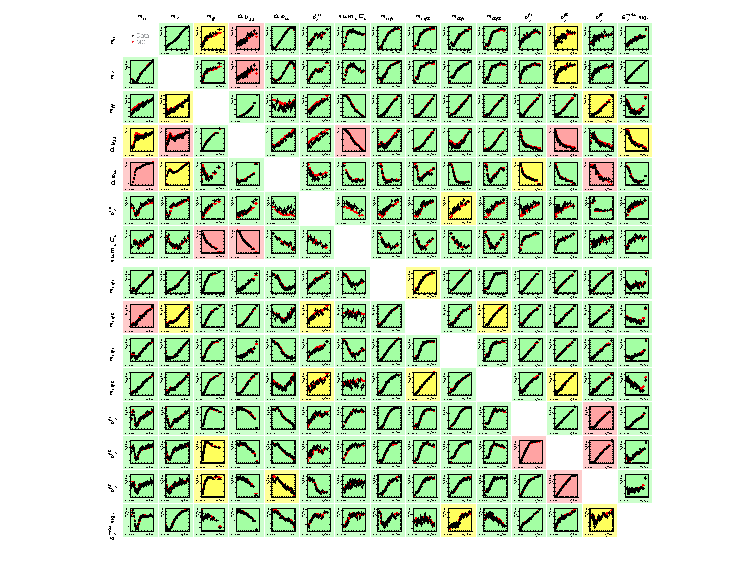
\includegraphics[width=\textwidth,trim=45 0 45 0]{figures/hww/dnn/correlations_PROF_SR.pdf}
    \caption{Visualization of the two-dimensional correlations between all combinations of DNN input variables, based on profiles of each of the distributions in the VBF-enriched \TwoJet SR. For all combinations of input variables $X_i$ and $X_j$, the distributions of both $\langle X_i \rangle$ vs $X_j$ and $\langle X_i \rangle$ vs $X_j$ are shown. The uncertainties are statistical only. The color for each plot encodes the $\chi^2$ probability, $p$, from the comparison: green represents $p > 0.05$, yellow represents $0.005 < p < 0.05$, and red represents $p < 0.005$.}
    \label{fig:dnn-features-profiles}
\end{figure}


\begin{figure}[t]
    \subfloat[] {
        \newImageResizeCustom{0.47}{figures/plots/feature-comparison.pdf}
    }
    \subfloat[] {
        \newImageResizeCustom{0.47}{figures/plots/arch-comparison.pdf}
    }
    \caption{VBF discovery significance for (a) different sets of variables and (b) different architectures of the neural network. The models trained with different architectures use the set of features corresponding to ``S4''. More information can be found in the text.}
    \label{fig:arch-vars-optim}
\end{figure}

% Include DNN figures (many plots!)
\dnnfigures


\begin{figure}[t]
    \subfloat[] {
        \newImageResizeCustom{0.48}{figures/hww/dnn/correlation-matrix-sig.pdf}
    }
    \subfloat[] {
        \newImageResizeCustom{0.48}{figures/hww/dnn/correlation-matrix-bkg.pdf}
    }
    \caption{Correlation matrix of the input features used in the VBF DNN for (a) the VBF signal and (b) the non-VBF-signal processes.}
    \label{fig:dnn-features-correlations}
\end{figure}


\subsection{Re-training the DNN and optimizing sample fraction}
\label{subsec:sample-fraction-optimization}
This is case in the VBF analysis, where systematic uncertainties of particular processes dominate the measurement uncertainties, and thus finding ways to train the DNN with putting more emphasis on the suppression of the processes with large uncertainties. 

Final optimization:
-  BKG weights (EWWW scan)!
-  Significances W/ and W/O syst uncertainties, W/ rebinning! (final optimization)

% Significance Z0:
% hww_syst_unc = {"Vgamma": 1, "otherVV":0.12, "Zjets": 0.25, "WW":0.3, "EWWW": 0.5, "singletop":0.5, "ttbar":0.3, "ggF":0.5, "VBF":0.3}


% Plots made with SFUsMLKit on cedar with:
% ./plot.py -c configs/HWW/winningSubmission.cfg --trainingFolderName dropout-02-5-fold-aggressive-lr-schedule-2-fine-scan-ewww-scan-etafix/210805_9_0.12_8226149877761426764
\begin{figure}[t]
    \subfloat[] {
        \newImageResizeCustom{0.47}{figures/plots/sample-fractions/sig_vs_lrate.pdf}
    }
    \subfloat[] {
        \newImageResizeCustom{0.47}{figures/plots/sample-fractions/sig_vs_ew_fraction_lr9.pdf}
    }
    \caption{}
    \label{fig:ew-fraction-scan}
\end{figure}

\begin{figure}[t]
    \subfloat[Without sample weighting] {
        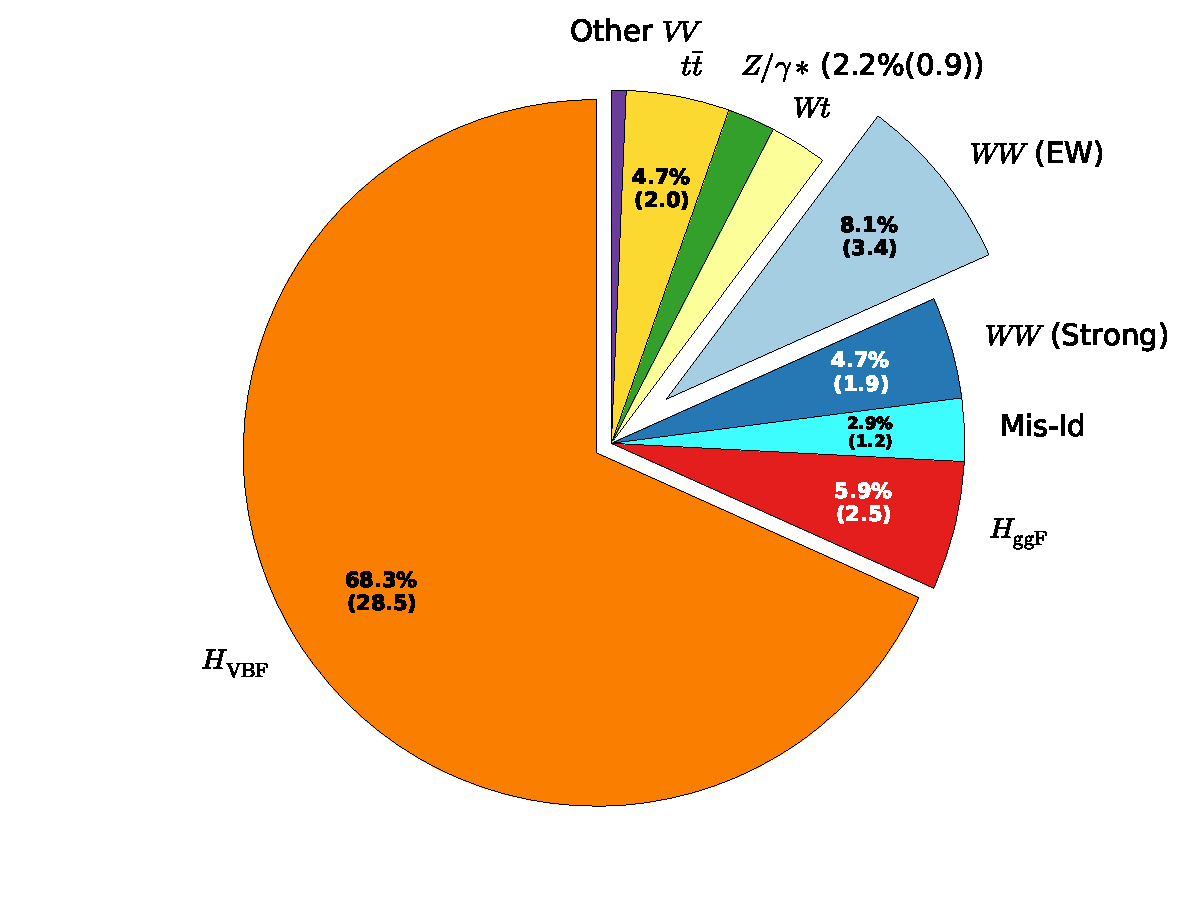
\includegraphics[width=0.5\textwidth,trim=45 0 0 0]{figures/plots/bkg-fraction-highest-bin/pie-chart-fractions-old.pdf}
    } 
    \subfloat[Optimized sample weighting] {
        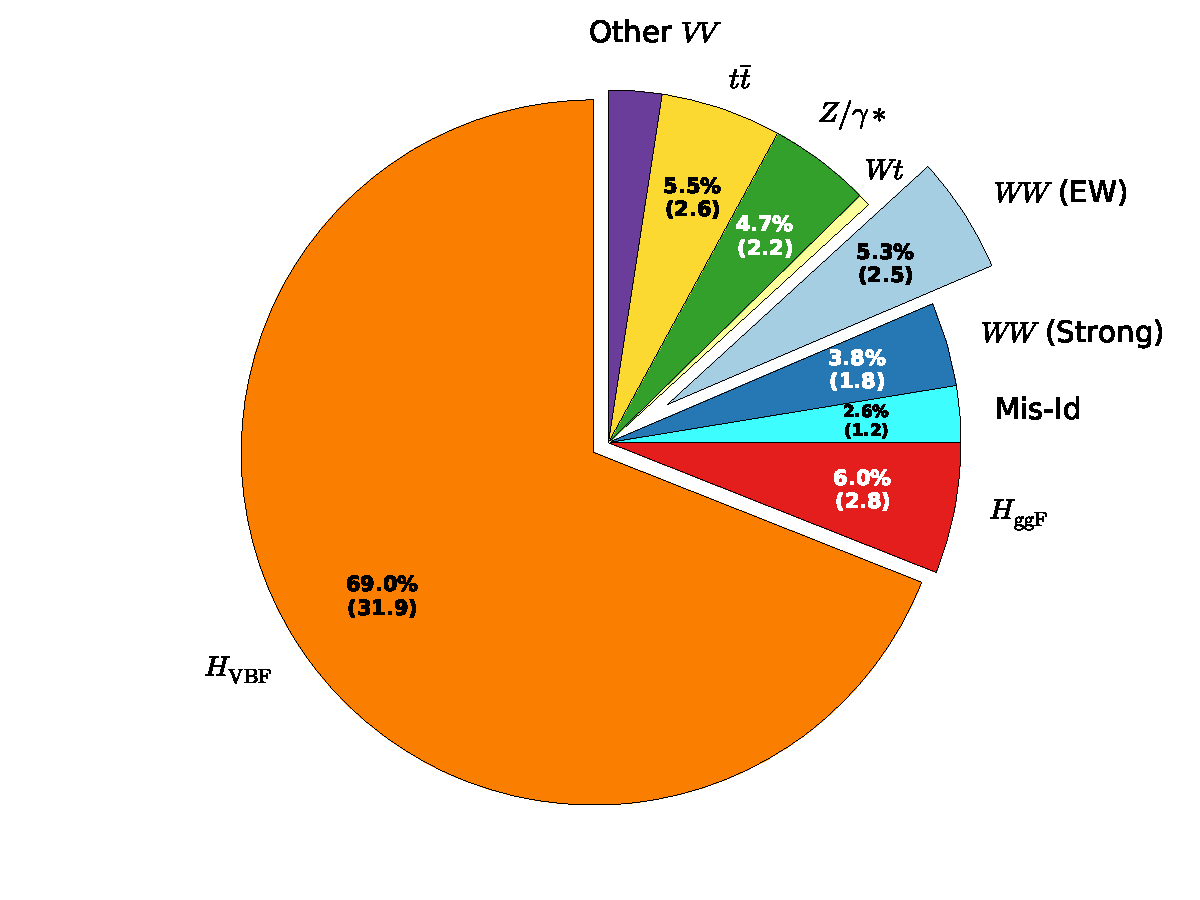
\includegraphics[width=0.5\textwidth,trim=45 0 0 0]{figures/plots/bkg-fraction-highest-bin/pie-chart-fractions-new.pdf}
    }
    \caption{Fraction of background in highest DNN output bin. }
    \label{fig:bkg-fractions}
\end{figure}


\subsection{Final model validation}

The distributions in \cref{fig:dnn-train-vs-test} show that the model generalizes very well.

- Plots with data (also LINEAR ONE! that was not approved by ATLAS? is that allowed?!)
\todo{Add plots of variables in different DNN bins!}


\begin{figure}[t]
    \subfloat[] {
        \newImageResizeCustom{0.49}{figures/hww/dnn/train_vs_test_dnn_score_normalized_log.pdf}
    }
    \subfloat[] {
        \newImageResizeCustom{0.49}{figures/hww/dnn/train_vs_test_dnn_score_zoom_non-normalized_non-log.pdf}
    }
    \caption{Comparison of the DNN output distributions of the training set and test set corresponding to the training data for (a) the full range of DNN output values and (b) the region with high VBF signal purity.}
    \label{fig:dnn-train-vs-test}
\end{figure}
